%
% Este template é baseado no template do pandoc 3.1.12.1.
% > pandoc -D latex
% Ele gera um trabalho acadêmico que respeita as normas da UFMG conforme o
% documento dispnível em:
% https://
%
% As modificações foram mantidas a um mínimo e buscou-se ao máximo somente
% acrescentar elementos novos, assim toda a documentação do pandoc permanece
% válida.
%

% Options for packages loaded elsewhere
\PassOptionsToPackage{unicode,pdfa}{hyperref}
\PassOptionsToPackage{hyphens}{url}
%
\pdfminorversion=7
%\special{pdf: minorversion 7}

\documentclass[
  12pt,
  a4paper,
  oneside,
  openright,
  sumario=abnt-6027-2012,
  english,
  brazil]{abntex2}

% PDFA Stuff
\usepackage[a-2b,mathxmp]{pdfx}[2018/12/22]
\begin{filecontents*}[overwrite]{jobname.xmpdata}
\Title{Título do documento}
\Author{Nome do autor}
\Language{en-US}
\Subject{Assundo do documento}
\Keywords{palavra chave, outra palavra chave, mais uma, assim vai},
\end{filecontents*}

\usepackage{amsmath,amssymb}
\usepackage{iftex}
\ifPDFTeX
  \usepackage[T1]{fontenc}
  \usepackage[utf8]{inputenc}
  \usepackage{textcomp} % provide euro and other symbols
\else % if luatex or xetex
  \usepackage{unicode-math} % this also loads fontspec
  \defaultfontfeatures{Scale=MatchLowercase}
  \defaultfontfeatures[\rmfamily]{Ligatures=TeX,Scale=1}
\fi
\usepackage[]{lmodern}
\ifPDFTeX\else
  % xetex/luatex font selection
\fi
% Use upquote if available, for straight quotes in verbatim environments
\IfFileExists{upquote.sty}{\usepackage{upquote}}{}
\IfFileExists{microtype.sty}{% use microtype if available
  \usepackage[]{microtype}
  \UseMicrotypeSet[protrusion]{basicmath} % disable protrusion for tt fonts
}{}
\makeatletter
\@ifundefined{KOMAClassName}{% if non-KOMA class
  \IfFileExists{parskip.sty}{%
    \usepackage{parskip}
  }{% else
    \setlength{\parindent}{0pt}
    \setlength{\parskip}{6pt plus 2pt minus 1pt}}
}{% if KOMA class
  \KOMAoptions{parskip=half}}
\makeatother
\usepackage{xcolor}
\usepackage{longtable,booktabs,array}
\usepackage{calc} % for calculating minipage widths
% Correct order of tables after \paragraph or \subparagraph
\usepackage{etoolbox}
\makeatletter
\patchcmd\longtable{\par}{\if@noskipsec\mbox{}\fi\par}{}{}
\makeatother
% Allow footnotes in longtable head/foot
\IfFileExists{footnotehyper.sty}{\usepackage{footnotehyper}}{\usepackage{footnote}}
\makesavenoteenv{longtable}
\usepackage{graphicx}
\makeatletter
\def\maxwidth{\ifdim\Gin@nat@width>\linewidth\linewidth\else\Gin@nat@width\fi}
\def\maxheight{\ifdim\Gin@nat@height>\textheight\textheight\else\Gin@nat@height\fi}
\makeatother
% Scale images if necessary, so that they will not overflow the page
% margins by default, and it is still possible to overwrite the defaults
% using explicit options in \includegraphics[width, height, ...]{}
\setkeys{Gin}{width=\maxwidth,height=\maxheight,keepaspectratio}
% Set default figure placement to htbp
\makeatletter
\def\fps@figure{htbp}
\makeatother
\setlength{\emergencystretch}{3em} % prevent overfull lines
\providecommand{\tightlist}{%
  \setlength{\itemsep}{0pt}\setlength{\parskip}{0pt}}
\setcounter{secnumdepth}{5}
% definitions for citeproc citations
\NewDocumentCommand\citeproctext{}{}
\NewDocumentCommand\citeproc{mm}{%
  \begingroup\def\citeproctext{#2}\cite{#1}\endgroup}
\makeatletter
 % allow citations to break across lines
 \let\@cite@ofmt\@firstofone
 % avoid brackets around text for \cite:
 \def\@biblabel#1{}
 \def\@cite#1#2{{#1\if@tempswa , #2\fi}}
\makeatother
\newlength{\cslhangindent}
\setlength{\cslhangindent}{1.5em}
\newlength{\csllabelwidth}
\setlength{\csllabelwidth}{3em}
\newenvironment{CSLReferences}[2] % #1 hanging-indent, #2 entry-spacing
 {\begin{list}{}{%
  \setlength{\itemindent}{0pt}
  \setlength{\leftmargin}{0pt}
  \setlength{\parsep}{0pt}
  % turn on hanging indent if param 1 is 1
  \ifodd #1
   \setlength{\leftmargin}{\cslhangindent}
   \setlength{\itemindent}{-1\cslhangindent}
  \fi
  % set entry spacing
  \setlength{\itemsep}{#2\baselineskip}}}
 {\end{list}}
\usepackage{calc}
\newcommand{\CSLBlock}[1]{\hfill\break\parbox[t]{\linewidth}{\strut\ignorespaces#1\strut}}
\newcommand{\CSLLeftMargin}[1]{\parbox[t]{\csllabelwidth}{\strut#1\strut}}
\newcommand{\CSLRightInline}[1]{\parbox[t]{\linewidth - \csllabelwidth}{\strut#1\strut}}
\newcommand{\CSLIndent}[1]{\hspace{\cslhangindent}#1}
%\ifLuaTeX
%\usepackage[bidi=basic]{babel}
%\else
%\usepackage[bidi=default]{babel}
%\fi
% get rid of language-specific shorthands (see #6817):
\let\LanguageShortHands\languageshorthands
\def\languageshorthands#1{}
%\ifLuaTeX
%  \usepackage{selnolig}  % disable illegal ligatures
%\fi
\usepackage{bookmark}
\IfFileExists{xurl.sty}{\usepackage{xurl}}{} % add URL line breaks if available
\urlstyle{same}
% Careful: hypersetup is going to be ignored if we use pdfx (and we do so for PDFa/ compliance)
\hypersetup{
  pdftitle={Título do documento},
  pdfauthor={Nome do autor},
  pdflang={brazil},
  pdfsubject={Assundo do documento},
  pdfkeywords={palavra chave, outra palavra chave, mais uma, assim vai},
  hidelinks,
  pdfcreator={LaTeX via pandoc}}

\author{}
\date{}

% --- Carrega o pacote ufmg-abntex2
\usepackage{ufmg-abntex2}

% --- Carrega o package necessário para a folha de aprovação
\usepackage{pdfpages}

% --- Instituição (o comando \imprimirinstituicao já é fornecido pela ABNTEX2)
\instituicao{Universidade Federal de Ciências}

% --- Faculdade (fornece \imprimirfaculdade, usado na capa e folha de rosto)
\faculdade{Faculdade de Ciências}

% --- Departamento
\departamento{Departamento de Ciência}

% --- Autor
\autor{Autor da Silva}

% --- Título
\titulo{Título Completo da Obra}

% --- Subtítulo
\subtitulo{Um subtítulo}

% --- Local
\local{Cidade do Trabalho}

% --- Data
\data{2024}

% --- Preambulo
\preambulo{Tese apresentada ao Programa de Pós-graduação em Ciência da
Universidade Federal de Ciências, como requisito parcial à obtenção do
título de Doutor em Ciências.}

% --- Orientador
\orientador{Orientador de Oliveira}

% --- Coorientador

\begin{document}

% --- Coorientador
\imprimircapa

% --- Folha de rosto e ficha catalográfica
\imprimirfolhaderosto*

% Imagem alinhada à direita e à margem inferior da página
\begin{fichacatalografica}
    \vspace*{\fill}
	\begin{flushright}
		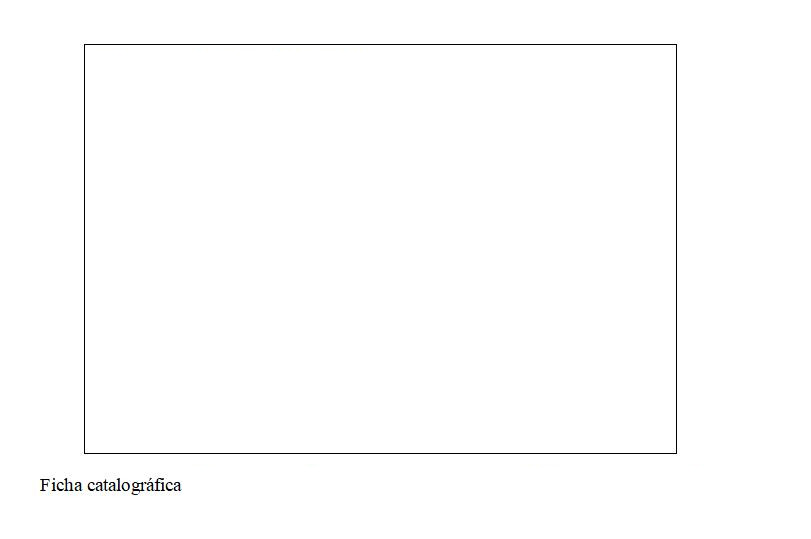
\includegraphics[]{fichacatalografica.jpg}
	\end{flushright}
\end{fichacatalografica}


% --- Aqui seria o local da errata (se alguém ainda usasse isso).

% -- Folha de aprovação

\includepdf{folhaaprovacao.pdf}

% --- Dedicatória
\begin{dedicatoria}
	Dedicado à toda a comunidade de sofware livre brasileira.
\end{dedicatoria}

% --- Agradecimentos
\begin{agradecimentos}
	Digite aqui seu texto de agradecimento. Cuidado para não esquecer
ninguém!
\end{agradecimentos}

% --- Epígrafe
\begin{epigrafe}
	Beware of bugs in the above code; I have only proved it correct, not
tried it. (Donald Knuth)
\end{epigrafe}

% --- Resumo em língua vernácula
\UFMGresumolinguavernacula{Este é o resumo do trabalho em língua
portuguesa. Você precisa também definir as palavras-chave em português.
Elas serão impressas logo abaixo. De acordo com as normas de UFMG, as
palavras-chave devem ser separadas por ponto-e-vírgula e finalizadas com
ponto final.}{primeira; segunda; terceira; palavra composta.}

% --- Resumo em lingua estrangeira (geralmente inglês)
\UFMGresumolinguaestrangeira{This work aims to contribute to the
community.}
{keyword1; keyword2; keyword3.}
{english}
{Abstract}
{Keywords}

% --- Lista de figuras
\pdfbookmark[0]{\listfigurename}{ldf}
\listoffigures*
\cleardoublepage

% --- Lista de tabelas
\pdfbookmark[0]{\listtablename}{lot}
\listoftables*
\cleardoublepage

% --- Lista de Siglas, abreviações e símbolos
\begin{siglas}
			\item[A] Primeiro símbolo ou sigla
				\item[B] Segundo símbolo ou sigla
				\item[C] Terceiro símbolo ou sigla
	\end{siglas}




{
\setcounter{tocdepth}{2}
\indent\tableofcontents*
\cleardoublepage
}


\textual

\chapter*{Introdução}\label{introduuxe7uxe3o}
\addcontentsline{toc}{chapter}{Introdução}

Texto da sua introdução.

\chapter{O melhor primeiro capítulo do
mundo}\label{o-melhor-primeiro-capuxedtulo-do-mundo}

Texto do seu primeiro capítulo. Você pode fazer citações ao estilo
Pandoc Markdown, como sugere HAUGELAND
(\citeproc{ref-haugeland1980}{1980}). Você pode também fazer citações
longas:

\begin{citacao}

Mea long citatio. Lorem ipsum dolor sit amet, consectetur adipiscing
elit, sed do eiusmod tempor incididunt ut labore et dolore magna aliqua.
Ut enim ad minim veniam, quis nostrud exercitation ullamco laboris nisi
ut aliquip ex ea commodo consequat. Duis aute irure dolor in
reprehenderit in voluptate velit esse cillum dolore eu fugiat nulla
pariatur. Excepteur sint occaecat cupidatat non proident, sunt in culpa
qui officia deserunt mollit anim id est laborum.
(\citeproc{ref-haugeland1980}{HAUGELAND, 1980, p. 45})

\end{citacao}

\chapter{O melhor segundo capítulo do
mundo}\label{o-melhor-segundo-capuxedtulo-do-mundo}

Texto do seu segundo capítulo. Se você ativar a lista de tabelas, uma
lista será montada automaticamente a partir de todas as tabelas que
forem encontradas no seu texto.

\begin{longtable}[]{@{}rlcl@{}}
\caption{Exemplo de uma tabela simples}\tabularnewline
\toprule\noalign{}
Direita & Esquerda & Centro & Padrão \\
\midrule\noalign{}
\endfirsthead
\toprule\noalign{}
Direita & Esquerda & Centro & Padrão \\
\midrule\noalign{}
\endhead
\bottomrule\noalign{}
\endlastfoot
A & A & A & A \\
B & B & B & B \\
\end{longtable}

\section{Uma seção dentro do segundo
capítulo}\label{uma-seuxe7uxe3o-dentro-do-segundo-capuxedtulo}

Texto da seção no interior do segundo capítulo.

\chapter{O melhor terceiro capítulo do
mundo}\label{o-melhor-terceiro-capuxedtulo-do-mundo}

Evidentemente, nem todas as funções disponíveis ao ABNTEX2 estão
contempladas no template que forneci aqui, então se você tem
necessidades outras, você sempre pode mexer diretamente no template
\emph{LaTeX}.

Este é um novo parágrafo, apenas para que você possa verificar o
distanciamento e a tabulação.

\begin{figure}
\centering

\includegraphics[width=2.08333in,height=\textheight]{ufmg.jpg}
\caption{Uma imagem}
\end{figure}

Acima temos uma imagem. Se você ativar a lista de imagens, o PDF gerado
conterá uma lista com todas as imagens identificadas no seu texto.

\section{Uma seção dentro do terceiro
capítulo}\label{uma-seuxe7uxe3o-dentro-do-terceiro-capuxedtulo}

Texto da seção no interior do terceiro capítulo.

\subsection{Uma seção dentro da seção do terceiro
capítulo}\label{uma-seuxe7uxe3o-dentro-da-seuxe7uxe3o-do-terceiro-capuxedtulo}

Texto da seção no interior da seção do terceiro capítulo.

\subsubsection{Uma seção dentro da seção da seção do terceiro
capítulo}\label{uma-seuxe7uxe3o-dentro-da-seuxe7uxe3o-da-seuxe7uxe3o-do-terceiro-capuxedtulo}

Você já entendeu.

\chapter*{Conclusão}\label{conclusuxe3o}
\addcontentsline{toc}{chapter}{Conclusão}

Este é um trabalhado não acabado, ao contrário do seu autor.

\phantomsection\label{refs}
\begin{CSLReferences}{0}{1}
\bibitem[\citeproctext]{ref-fodor1980}
FODOR, J. A. \textbf{The language of thought}. Harvard University Press,
1980.

\bibitem[\citeproctext]{ref-haugeland1980}
HAUGELAND, J. Programs, causal powers and intentionality. \textbf{The
Behavioral and Brain Sciences}, v. 3, p. 432--433, 1980.

\end{CSLReferences}

\end{document}
